Following our preference for simplicity, we propose a three-stage architecture, shown in figure \ref{fig:architecture-stateestimation}. Measurements arriving from different sensors are first preprocessed, which, for example, includes unit conversions and coordinate transformations. In the next steps, outliers are detected. The outlier state informs the fusion of the measurements into an accurate state estimate (requirement 1) through an \gls{ekf}, which is then used by the subsequent \gls{vdc}'s performance components and \gls{dv} software.

\begin{figure}
	\centering
	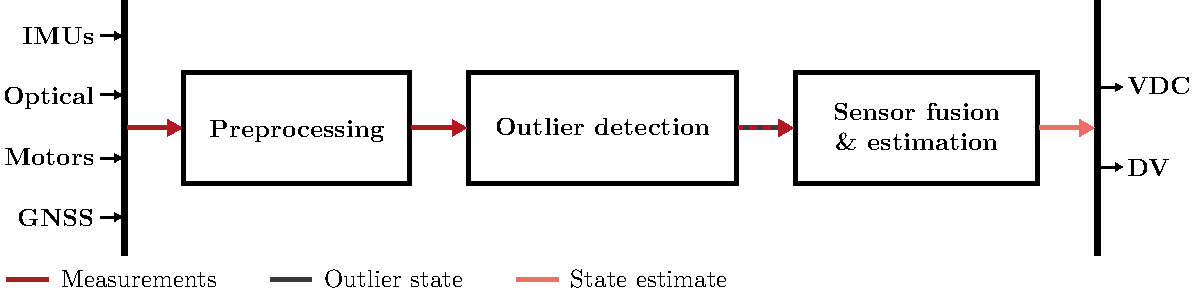
\includegraphics[width=\textwidth]{architecture_stateestimation}%
	\caption{Architecture of state estimation}
	\label{fig:architecture-stateestimation}
\end{figure}

A key feature is the unified mechanism for outlier and sensor setup detection (requirements 2 and 3). Foundation is the realization that ultimately it does not matter if a measurement is unavailable due to an invalid signal or a missing sensor, therefore both cases can be treated the same. This allows a focused effort on a single component while reducing complexity. Still, the name \textit{outlier detection} will be used. The following sections describe each of the three component in detail.


\subsection{Preprocessing}
Goal of the preprocessing stage is to harmonize all measurements and pre-fuse them for the subsequent estimation stage. Mostly, this is only a simple conversion to SI units, e.g., velocities from \si{\kilo\meter\per\hour} to \si{\meter\per\second}, or angles from \si{\deg} to \si{\radian}. Doing these conversions as early as possible simplifies subsequent computations and reduces error potential due to wrong units. For other signals, more preprocessing is necessary.

\begin{description}
\item[IMU] The most sophisticated preprocessing is required for the \glspl{imu}. The measurements are first rotated in three dimensions to correct any misalignment with the vehicle axes. This calibration must be performed every time the sensor orientation is changed. Then, we need a generic \gls{imu} fusion algorithm which can take an arbitrary number of sensors with known positions and fuse them into an estimate of the state variables $a_x$, $a_y$, $\dot{\psi}$ and $\ddot{\psi}$. An accurate estimate of these variables is important, because they are extensively used in the sensor fusion and performance components. This helps with reducing noise, but also enables calculation of the angular acceleration, which cannot be measured directly with our sensors. We always calculate the linear acceleration and angular velocity in three dimensions, and, in case of more than two \glspl{imu}, the angular acceleration as well. We provide two approaches for \gls{imu} fusion with the same interface, enabling drop-in replacement. Since the available \glspl{imu} need to be known at this point, performing the outlier detection here instead of the outlier detection state is necessary.

The first approach fuses measurements by averaging, and is therefore called \textit{mean-based \gls{imu} fusion}. First, the angular velocity measurements from the gyrometers are averaged. Then, the angular accelerations are derived using equation \ref{eq:angacc-from-linacc-3d} from all combinations of two \glspl{imu} and averaged. For example, in the \gls{ev}, the combinations 1--2, 2--3 and 1--3 are regarded. In case only two \glspl{imu} are available, they are assumed to have a zero $z$-position and the angular acceleration is calculated using the simplified equation \ref{eq:angacc-from-linacc-2d}. In case only a single \gls{imu} is available, we assume $\alpha = \mathbb{0}$. Finally, the linear accelerations are transformed to the \gls{cog} using equation \ref{eq:offcenter-acceleration-3d} and averaged as well, which eliminates the effect of tangential and centripetal acceleration.

The second \textit{maximum-likelihood-based \gls{imu} fusion} approach is more sophisticated and is presented in \cite{Skog.2016}, with an extension proposed in \cite{Wahlstrom.2018}. The idea is to first find a maximum-likelihood estimate for $\omega$ given the linear acceleration and angular acceleration measurements of all sensors. This is done by solving a least-squares problem using the Gauss-Newton algorithm, with a fixed number of 10 iterations instead of checking for convergence. The maximum-likelihood estimate for $a$ and $\alpha$ is then as simple as plugging the previously found estimate into a linear equation.

\item[Optical velocity sensor] The optical cross-correlation velocity sensor is located on the right side behind the \gls{cog}, so its measurements need to be corrected to account for the component induced by a yaw rotation. Equation \ref{eq:offcenter-velocity-2d} is used to transform the measurements to the \gls{cog}. Note that the yaw rate is required, so a direct signal from the \gls{imu} preprocessing is required.

\item[Motor speed sensor] The motor rotation speeds are used as another vehicle velocity source via equation \ref{eq:wheelspeeds}, averaging over all four wheels to fuse them as described in section \ref{sec:motorspeeds-to-velocity}.

\item[\gls{gnss}] Position measurements from the \gls{gnss} arrive in latitude-longitude-height coordinates, but need to be transformed to topocentric east-north coordinates, i.e. coordinates on a plane tangential to the earth at a certain reference point~\cite[p.~475 f.]{Grewal.2007}. The transformation is based on the ellipsoid WGS 84 earth model used in \gls{gps} measurements. The reference point is the first known position, and all future positions will be represented in $x$-$y$-coordinates relative to the reference point.

Only speed measurements are available through \gls{gnss}, i.e. the absolute value of the velocity. However, since the vehicle sideslip angle $\beta$ is usually small and less than \SI{0.1}{\radian}, the longitudinal velocity can be approximated to be the speed, i.e. $v_x \approx \norm{v}$ and $v_y \approx 0$. This simplification works well in our design, since the \gls{gnss} speed will only be used for outlier detection, not as part of the final state estimate. If separate measurements for the eastward and northward velocity become available, they can be transformed into vehicle coordinates using equation \ref{eq:transform-linear-velocity}. Note that this requires heading information, which might not always be available.
\end{description}


\subsection{Outlier Detection}
Our approach towards outlier detection is heavily based on the dual method presented in section \ref{sec:outlier-types}, to help minimize both false-positives and false-negatives. The complete outlier detection stage is shown in figure \ref{fig:architecture-outlierdetection}. It receives signals from the preprocessing stage and determines the binary sensor state (OK, NOT OK), i.e. whether the sensor is available and does not contain outliers. The target is to support one sensor failure, since more are unlikely.

\begin{figure}
	\centering
	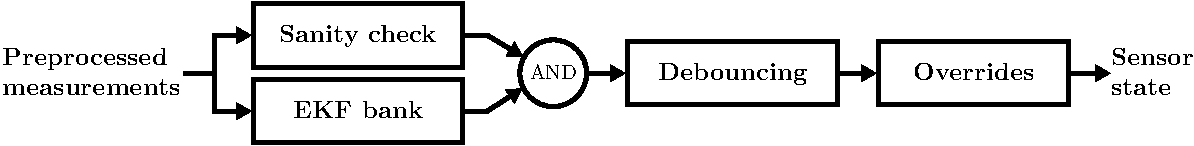
\includegraphics[width=\textwidth]{architecture_outlierdetection}%
	\caption{Architecture of outlier detection}
	\label{fig:architecture-outlierdetection}
\end{figure}

Every input for the estimation stage undergoes a sanity check, presented in equations \ref{eq:outlier-range} and \ref{eq:outlier-maxchangerate}. This is also the outlier detection method performed to select the \glspl{imu} for the \gls{imu} fusion. The range of the signal and the difference to the last sample are checked for plausibility, and the time since the last sample is used to detect a sensor timeout. This is also the mechanism to detect the sensor setup, because missing sensors will timeout permanently. While we described many other methods in section \ref{sec:outlier-statisticalmethods}, we chose the simplest method with the least parameters.

Accurate knowledge of the vehicle velocity is of special importance for the performance component. Since we have three velocity sources, we can apply the \gls{ekf} bank approach from equation \ref{eq:outlier-ekfbank}. We run three \glspl{ekf} in parallel using the model presented in the next section. For each \gls{ekf}, one sensor is disabled, so the other \glspl{ekf} generate high residuals in case of a failure of that sensor. This case is checked by comparing the normalized sum of squared residuals with a threshold. The covariance of all velocity measurements is identical to ensure equal weighting. This is necessary to detect persistent outliers, since residuals caused by outliers would otherwise quickly return to zero even if outliers persist because the low-covariance measurements pull the estimate towards the faulty value. Note that successful fault isolation requires at least three measurements, otherwise only fault detection is possible. Because velocities are also checked by the \gls{ekf} bank, their plausibility check is configured to be rather lenient.

The results from the sanity check and the \gls{ekf} bank are logically and-ed, with OK for the results of non-velocities from the \gls{ekf} bank. Detected outliers are then debounced to increase robustness in case outliers appear and disappear quickly. Debouncing means that a signal is marked as NOT OK for a certain span of time after an outlier has been detected, even if no outlier is currently detected. Only if the time span passes without another outlier, the signal is marked as OK once again.

Last in the chain is a three-way override for each signal. Either the outlier state can be directly forwarded, or forced to be OK or NOT OK. On the one hand, this allows to correct erroneous detection results, on the other hand it also provides a way to manually enable and disable sensors in case the sensor setup detection fails.

\subsection{EKF}
imu fusion for a, omega, alpha
EKF for remaining state variables, but takes IMU stuff as input
outlier detection sensor state and dt signal is used to create measurement mask (requirement 4)
Show input selection and state equations, jacobians
euler forward discretization
GPS is not included because it is not beneficial due to its slow response, only when no wheels and kistler
kinematic model from~\cite[p.~156]{AlexanderWischnewski.2019}
simple without tire model: occams razor and empiric by wisch
reduces effects of noise
no heading measurements in ev, especially lack of initial heading is bad
normalize angles
equation for dv based on \ref{eq:cornering-acceleration}

prediction using differential equation
initialization
disable measurements using separate mask
input cov as process noise
